% !TEX root = BA-Bericht.tex
\chapter{Realisierung}
% TODO Beschreibung der Umsetzung der definierten Ziele, einschliesslich der aufgetretenen Schwierigkeiten und Einschränkungen

% Dies ist das Hauptkapitel Ihrer Arbeit! Hier wird die Umsetzung der eigenen Ideen und Konzepte
% (Kapitel 3) anhand der gewählten Methoden (Kapitel 4) beschrieben, inkl. der dabei aufgetretenen
% Schwierigkeiten und Einschränkungen.

Dieses Kapitel beschreibt wie die definierten Ziele umgesetzt werden.
Zudem wird erwähnt wo Schwierigkeiten aufgetreten sind 

In den Abschnitten \fullref{sec:real_projektmanagement}

\section{Projektmanagement}\label{sec:real_projektmanagement}

Die folgenden Unterkapitel zeigen kurz auf wo das Projekt an den definierten Meilensteinen stand.
Zudem wird erklärt warum gewisse Ziele nicht erreicht wurden. Auch wird aufgezeigt was für Massnahmen getroffen wurden, um das Projekt wieder auf den richtigen Weg zu bringen.

\subsection{Meilenstein 1: Grobkonzept}

Zu diesem Zeitpunkt habe ich ein Grobkonzept erstellt, welches aufzeigt wie ich grob die Aufgabenstellung zu lösen bedenke.
Jedoch bin nach dem Arbeitsjournal ich etwa zwei Arbeitstage im Rückstand und der Stand der Technik wurde zwar recherchiert aber noch nicht in den Bericht niedergeschrieben.
Wir haben nach diesem Meilenstein beschlossen, dass ich in das Büro der Kopanyo AG arbeiten kann aufgrund der erheblichen Lärmemissionen bei mir Zuhause im Home-Office. Dies hat es extrem schwierig gemacht sich zu konzentrieren und bei der Sache zu bleiben.

\subsection{Meilenstein 2: Zwischenpräsentation}

Während die Zwischenpräsentation ein voller Erfolg war, war der Teststand zu diesem Zeitpunkt noch nicht fertig gestellt. Auch bin ich etwa zweieinhalb Arbeitstage im Rückstand was das Arbeitsjournal aufzeigt.

Die Zwischenpräsentation war ein voller Erfolg und ich habe viele positive Rückmeldungen erhalten.
Zudem noch einige vom Experten Hinweise was es zu beachten gilt bei Latenzmessungen.

Jedoch konnte ich meinen Teststand noch nicht demonstrieren, da ich noch Probleme mit der Netzwerkkonfiguration des neueren Docker-Compose Ansatzes habe.

\subsection{Meilenstein 3: Auswertung}

Zum Zeitpunkt dieses Meilensteins konnte der Teststand sowie die Messanlage grösstenteils fertiggestellt werden und ich konnte erste Latenzmessungen mit Nachrichten im Netzwerk durchführen.
Jedoch wird das 

\subsection{Meilenstein 4: Web-Abstract}

\subsection{Abgabe}
Diese Liste von Resultaten ist auch ein guter Ausgangspunkt um davon Issues für den Issue-Tracker zu erstellen.
Jeder issue kann nun auch sortiert werden nach Resultat-Kategorien z.B. ''Recherche'', ''Projektmanagement'', ''Dokumentation'', ''Evaluation'', ''Präsentation'', etc.

\section{Systemarchitektur}\label{sec:systemarchitektur}

Wie Kapitel~\fullref{ch:ideen_und_konzepte} wurde konzeptionell ausgeführt die der Teststand und die Messanlage für das I2P-Testnetzwerk aussehen soll.
In diesem Abschnitt wird nun die resultierende Softwarearchitektur aufgezeigt.
Die entwickelte Software besteht grob aus fünf Teilen:

\begin{enumerate}
    \item \textbf{Deployment:} Hier ist die Deployment-Konfiguration für die Test-VM zu finden. Mittels NixOps kann dieselbe Test-VM reproduzierbar erstellt werden.
    \item \textbf{Test-VM \& deren Deployment}: Die Test-VM stellt eine reproduzierbare und isolierte Umgebung zur Verfügung, um darin die Messungen durchführen zu können.
     Die Virtuelle Maschine grenzt die Ressourcen des Testnetzwerks klar ein.
     Es handelt sich hier um ein Linux-System welches Docker installiert hat,
	 um darin die benötigen Container zu erstellen.
    \item \textbf{Container-Deployment}: Dieser Bestandteil ist verantwortlich die anhand der Testkonfiguration das I2P-Testnetzwerk, inklusive den Shared-Volumes, mit Hilfe von Docker zu erstellen. Dazu wird das \lstinline|recompose|-Skript verwendet.
	 Hierbei handelt es sich um einen Wrapper, der intern docker-compose verwendet.
    \item \textbf{I2P-Testnetzwerk:} Das Testnetzwerk besteht aus i2pd-Containern sowie aus dem Reseed-Container. Dieser wird benötigt wird, um das Testnetzwerk zu bootstrappen.
    \item \textbf{Messanlage:} Die Messanlage besteht aus einem TCP-Server und TCP-Client die zusätzlich in den i2pd-Containern angesiedelt sind.
        Zudem gibt es ein Messskript welches den Nachrichtenversand vom TCP-Client zum TCP-Server anstossen kann und die Messresultate sammelt.
\end{enumerate}

Die Abbildung~\fullref{fig:architektur-diagramm} zeigt in einem Komponenten-Diagram die Systemarchitektur auf.

\begin{figure*}[htp]
  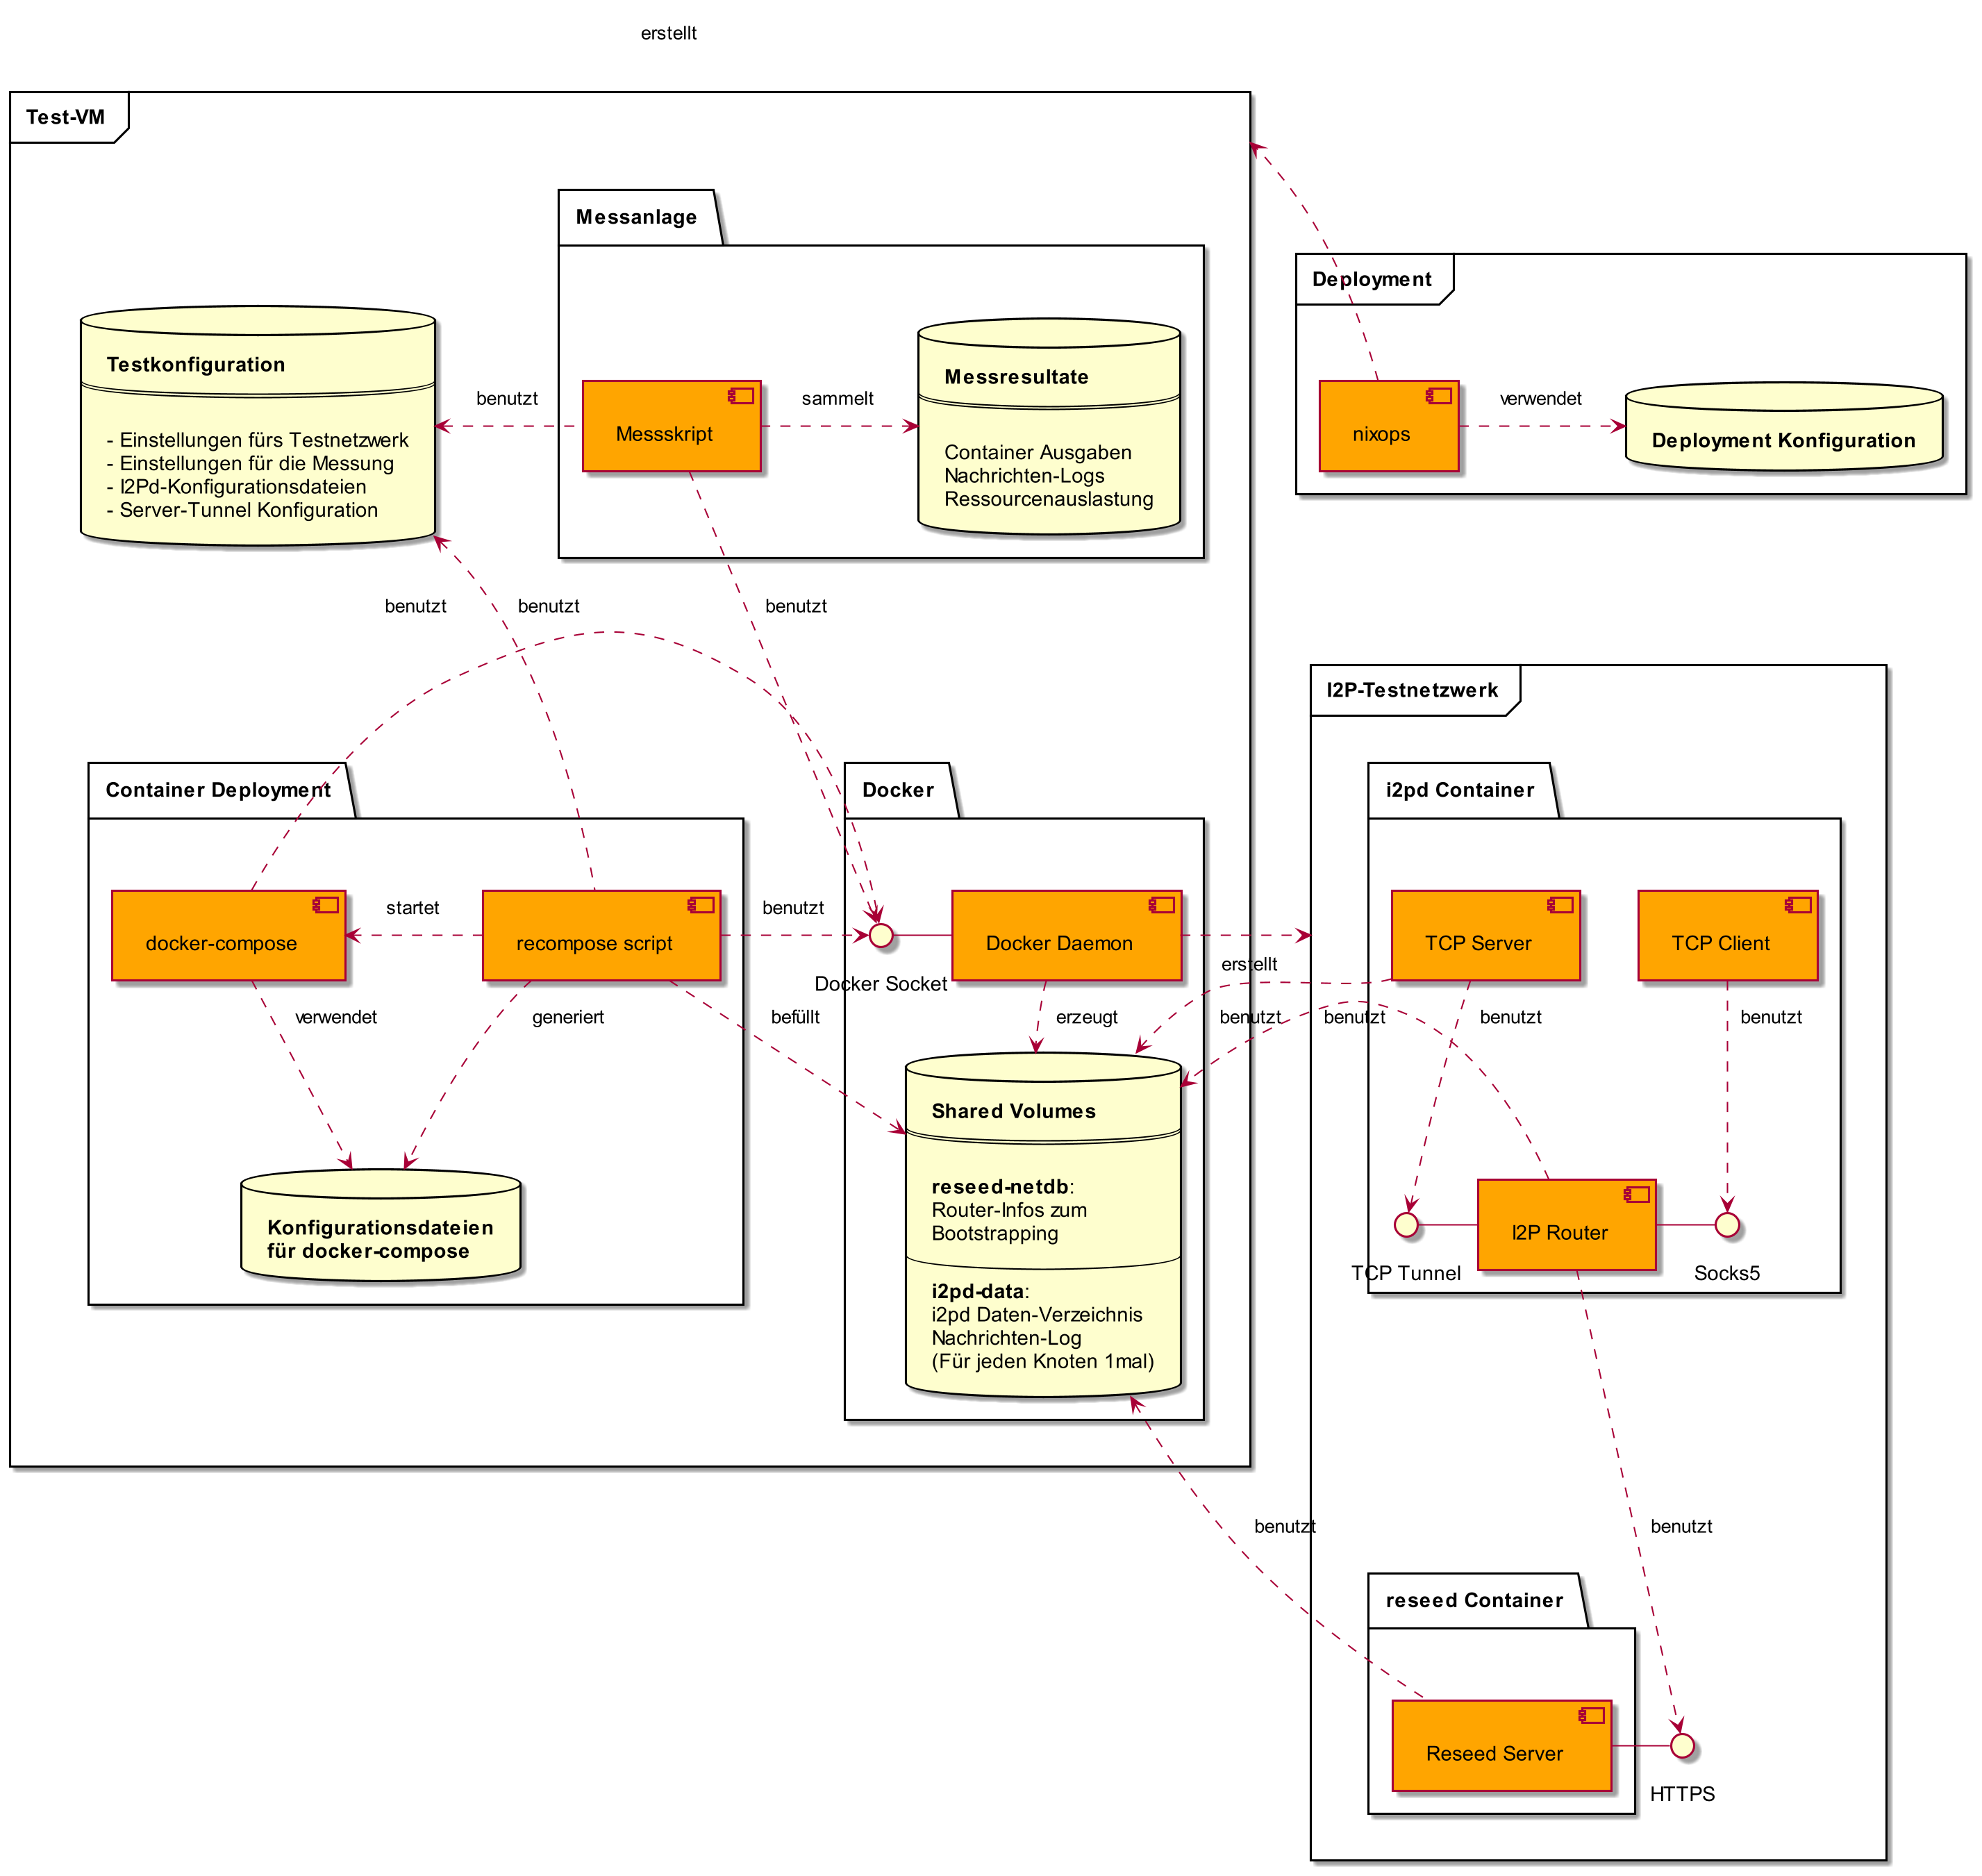
\includegraphics[width=1.1\textwidth]{include/uml/componentDiagram.png}
  \caption{Architektur-Diagramm}\label{fig:architektur-diagramm}
\end{figure*}


\section{Komponentendesign}\label{sec:komponentendesign}

In diesem Abschnitt werden die einzelnen Komponenten, wie aufgezeigt der Abbildung~\fullref{fig:architektur-diagramm}, genauer beschrieben.

\subsection{Deployment}

NixOps erlaubt es mittlels einer NixOS-Systemkonfiguration ein komplettes Linux auf diverse Arten von Maschinen zu deployen. Dies kann physische Hardware oder wie auch in diesem Falle eine VM sein.

Anstatt die Maschine

\subsection{Konfiguration}

Die Konfiguration des Teststands kann mittels einer json-Konfigurationsdatei einfach angepasst werden.
Da es sich hier um eine JSON-Datei handelt, kann diese falls nötig einfach von verschiedenen Programmen gelesen werden.
Einerseits wird diese vom Messkript gelesen, wie aber auch vom recompose Skript.


\subsection{Recompose-Skript}

Das Recompose-Skript ist dafür verantwortlich das Docker-Netzwerk anhand der Konfiguration aufzubauen und zu verwalten.
Es ist das Kernstück der entwickelten Software.

Es handelt sich hier um einen Wrapper um \lstinlline|docker-compose|

Als wichtigster Punkt wird hier der 

\subsection{Deployment der Knoten}

Die I2P-Knoten werden mittels docker-compose deployed.
\lstinline|docker-compose| erlaubt das automatisierte erstellen und abbauen von Netzwerken bestehend aus mehreren Docker-Containern.
Dazu liest \lstinline|docker-compose| jeweils eine oder mehrere YAML-Dateien.
In diesen YAML-Dateien können die verschiedenen Container, Netzwerke und Volumes und diverse Optionen deklariert werden, welche das zu erstellende Container-Netzwerk beschreibt.

Anfangs wurde versucht die Knoten unter Verwendung des \lstinline|scale|-Features zu skalieren.
Unter Verwendung dieses Feature muss der \lstinline|i2pd|-Knoten nur einmal deklariert werden und kann beim ausführen des \lstinline|docker-compose|-Befehls mehrfach instanziiert werden.
Jedoch hat dieses Feature zu Problemen geführt, sodass die \lstinline|i2pd|-Knoten nicht untereinander kommunizieren konnten.
Es kann gut sein das dieses Feature nicht für P2P-Netzwerke geeignet ist, da dieses normalerweise gebraucht wird um z.B. Datenbank- oder Webserverinstanzen zu skalieren.
Diese müssen normalerweise auch nicht untereinander kommunizieren.
Ausserdem verweist die Dokumentation auch immer mehr auf docker-swarm, um Knoten zu skalieren.

Schlussendlich wurde eine Lösung für dieses Problem gefunden,
indem das \lstinline|recompose|-Skript ein Teil der YAML-Konfiguration beim Ausführen generiert.
Für jeden Knoten der im Netzwerk sein sollte wird ein neuer Knoten deklariert.

% TODO: Referenziere generieren der Knoofen-Konifugrationen

\subsection{Deployment von der Container}

Da ich bereits NixOps zum deployment der Container verwendet habe, schien es naheliegend die NixOS-Container Technologie zu verwenden.

Jedoch bin ich mit diesem Ansatz an mehreren Stellen an Grenzen gestossen.

Als erstes traten Probleme mit der Netzwerkkonfiguration. Die NixOS-Container implementation scheinte die 

• Erst Probleme mit der Netzwerkkonfiguration
• Probleme mit Docker-Kompatibilität
• Skaliert nicht auf mehr als ein paar dutzend Container. Zu viel
RAM benötigt lediglich zum Berechnen der verschiedenen
Container-Konfigurationen.

Es hat 

Anfangs wurde auf ein Ansatz mit 


\subsection{Skalierung der i2pd-Container}

Der erste Lösungsansatz mit NixOS-Containern hat sich als ungeeignet herausgestellt. \seereq{TSCL}

Dieser Ansatz wurde verworfen, weil dies dazu geführt hat, das die i2pd-Container untereinander nicht kommunizieren konnten.

\subsection{Reseed-Server und Bootstrapping}

Die I2P-Router im öffentlichem I2P-Netzwerk können sich hier einfach an den öffentlich verfügbaren Reseeder eine \lstinline|su3|-Datei via HTTPS herunterladen.
Diese \lstinline|su3|-Datei beinhaltet RouterInfos. 
Diese RouterInfos beinhalten die nötigen Informationen wie public-key und Netzwerkadresse, um die Kommunikation zu starten.

Im privaten und abgeschotteten Testnetzwerk sind die öffentlichen Reseed-Server jedoch nicht erreichbar.
Deshalb muss ein anderer Weg gefunden werden das private I2P-Netzwerk zu bootstrappen.

Denn der Floodfill-Anstatz entspricht nicht unbedingt der Realität, denn die Reseeder-Knoten können liefern nicht allen I2P-Routern dieselbe Liste an Peers.

Auch kann die Konfiguration des Reseeders eine wichtige Rolle spielen, denn dieser bestimmt mit der Liste an Peers die er den I2P-Routern liefert den Konnektivitätsgrad der Knoten.

\subsection{Resultate zurücklesen}

Just read logs? Use some Docker cp magic?

\section{Umsetzung}\label{sec:umsetzung}

In diesem Abschnitt wird nun beschrieben,
wie die im vorherigen Abschnitt aufgezeigte \nameref{sec:systemarchitektur} und das dazugehörige \nameref{sec:komponentendesign} schlussendlich effektiv umgesetzt wurde.
Zudem wird der Weg zur schlussendlichen Lösung genauer beschrieben.
Zuerst wurde versucht ein Prototyp für das I2P-Testnetzwerk unter Verwendung von NixOS-Containern zu erstellen (siehe \nameref{sec:la1_nixos}).
Jedoch wurde schlussendlich eine andere Lösung gefunden, welche den Anforderungen gerecht wurde, unter Verwendung von Docker-Compose.
Der erzeugte Quellcode zur Erstellung des I2P-Testnetzwerk's sowie der Quellcode für die Messanlage ist im folgenden Repository zu finden:

\url{https://codeberg.org/mkuettel/i2p-testnet}


\section{Lösungsansatz: NixOS-VMs und NixOS-Container}\label{sec:la1_nixos}

Zu beginn des Projekts wurde versucht ein I2P-Testnetzwerk aufzubauen mit Hilfe von NixOps.
NixOps ist ein Tool zum Deployment von Netzwerken bestehend aus NixOS-Maschinen.
\cite{noauthor_nixops_nodate-5}
% Für genauere Anweisungen und weitere Möglichkeiten welche durch nixops geboten werden, siehe das ``NixOps User's Guide''\footnote{\url{https://releases.nixos.org/nixops/nixops-1.5/manual/manual.html}}.

NixOS ist eine Linux-Distribution basierend auf dem Paket-Manager Nix.
Nix erlaubt es reproduzierbare Softwarepakete zu erzeugen und kann mit einer deklarativen und funktionalen Programmiersprache konfiguriert werden.
% TODO: reference nix
Dieser Ansatz wurde zu Beginn aus mehreren Gründen ausgewählt.
Einerseits setze ich auch selber NixOS seit mehreren Jahren ein und NixOps ist somit das native Deployment-Tool.
Andererseits Nix legt enormen Wert auf Reproduzierbarkeit und das gesamte Netzwerk bis hin zum OS könnte anhand einer Nix-Konfiguration wiedererstellt werden.
Auch könnten Konfigurationen für I2P-Knoten wiederverwendet werden, egal ob diese nun in Container,
VMs oder auf echter Hardware deployed werden.
Dies ist möglich da System-Konfigurationen oder Teile davon bei NixOS unabhängig von der Konfiguration der effektiven Infrastruktur sind.
Ich habe angefangen mit NixOps ein Netzwerk bestehend aus einzelnen VirtualBox-VM zu erstellen.
Um weniger Ressourcen-Overhead zu haben, habe ich dann angefangen mehrere I2P-Knoten als NixOS-Container innerhalb dieser VM zu erstellen.
Auch habe ich damit angefangen eine Lösung für das Bootstrapping Problem zu finden.
Jedoch bin ich mit diesem Ansatz immer wieder an verschiedenen Stellen auf Probleme gestossen:

\begin{itemize}
    \item \textbf{Netzwerkkonfiguration:} Die Knoten konnten nicht korrekt untereinander kommunizieren. Es war nicht möglich einen anderen Container mittels einem \lstinline|ping|-Befehl zu erreichen.
        Es hat sich herausgestellt, dass das Routing zwischen den Containern sowie die Netzwerkmasken nicht korrekt konfiguriert wurden und es keine Option gab diese Routen richtig zu setzen innerhalb der Nix-Deklaration.
        Aufgrund dessen habe ich das NixOS-Modul für NixOS-Container erst selbst angepasst.
        Somit konnte ich die Routing-Probleme beheben und Optionen hinzufügen, um die Netzwerkmasken der Knoten korrekt zu setzen. %TODO: reference commit
        Das NixOS-Container Modul scheint also nicht ausgereift zu sein.
    \item \textbf{Docker-Kompatibilität:} Auch habe ich versucht anstatt von NixOS-Containern, Docker-Container auf NixOS zu erstellen.
        Dies hätte es erlaubt die bestehenden Container von DIVA.EXCHANGE wiederzuverwenden. Jedoch schien der Support für Docker auch nicht ausgereift genug.
        Ich konnte auf meinem Laptop keine Docker-Images bauen für das Testnetzwerk, da dies libvirt/QEMU-Support benötigt.
        Dies war unter gleichzeitiger Verwendung von VirutalBox nicht möglich, da nur ein Hypervisor gleichzeitig ausgeführt werden kann.
        Auch habe ich versucht den Hypervisor auf libvirt/QEMU zu wechseln, was aber schon am deployment der VM scheiterte.
    \item \textbf{Skalierungsprobleme:} Während dem entwickeln habe ich jeweils 2 oder 8 Knoten auf einmal erstellt, um schnell ein Feedback zu erhalten.
        Um den Reseeder zu testen hatte ich jedoch auf einmal versucht 103 Knoten zu erstellen.
        Jedoch hat nur schon das generieren und auswerten der NixOS-Systemkonfigurationen für alle diese NixOS-Container extrem viel Arbeitsspeicher benötigt.
        Meine 16GB Arbeitsspeicher in meinem Laptop wurden nach mehreren Sekunden gefüllt. Ich konnte somit die Knoten nicht einmal erstellen und deployen, da nur schon das berechnen der NixOS-Systemkonfigurationen zu ineffizent implementiert ist.
\end{itemize}
Somit war klar das dieser Lösungsansatz nicht funktionieren konnte und es musste ein grundsätzlich anderer Ansatz zur Erstellung der Container gefunden werden.

\section{Lösung mit Docker-Compose}

Nachdem sich herausgestellt hat, das der Lösungsansatz mit NixOS-Container nicht funktioniert, wurde eine Container-Orchestration Lösung gesucht.
Um unnötige Komplexität zu vermeiden wurde auf das einfache Tool \lstinline|docker-compose| gesetzt.
Zudem hat der Auftraggeber bereits Erfahrungen mit diesem Tool gemacht und es auch schon eingesetzt um i2pd-Netzwerke zu erstellen
für die Entwicklung an der DIVA-Blockchain.
Anhang \lstinline|docker-compose.yml|-Datei vom Auftraggeber,
konnte ein kleines öffentliches I2P-Testnetzwerk mit acht festkodierten i2pd-Container werden.
Dies wurde anschliessend als Ausgangspunkt verwendet.

\subsection{Skalierung}\label{sec:scaling}

Damit verschiedene Anzahl an I2P-Knoten im privaten Testnetzwerk getestet werden können, müssen diese skaliert werden können.
Anfangs wurde versucht auf die Skalierungsfunktion von \lstinline|docker-compose| zurückzugreifen.
Mittels der \lstinline|--scale|-Option des \lstinline|docker-compose up| Befehls, kann aus einem einzigen deklarierten Container mehrere Container instanziiert werden. Man kann diesen also nur einmal definieren, wie aufgezeigt in folgendem Listing:
\begin{lstlisting}{language=yaml}
# ... 
services:
  i2pd:
    build:
      context: "./docker/i2p"
    environment:
      ENABLE_TUNNELS: 1
    networks:
      i2ptestnet:
        ipv4_address: "10.23.128.1"
# ...  
\end{lstlisting}

Jedoch bin ich mit diesem Ansatz auf Netzwerkprobleme gestossen,
sodass die \lstinline|i2pd|-Container nie untereinander direkt kommunizieren konnten.
Die Vermutung besteht, dass diese Skalierungsfunktion nicht für P2P-Netzwerke gedacht ist.
Denn im Normalfall wird diese wohl verwendet ein Service auf einem Tier zu skalieren.
Beispielsweise kann damit ein App-Server-Prozess skaliert werden, welche aber natürlich nie untereinander kommunizieren müssen.
Dieses Problem wurde schlussendlich so gelöst,
dass nun dynamisch für jeden zu erstellenden Knoten eine\lstinline|i2pd|-Container-Deklaration anhand eines JSON-Template generiert wird.
Dieses JSON-Template ist in \lstinline|docker/i2p-node-base.json| zu finden.
Die fehlenden Werte, so wie z.B. eine statische IP, werden beim ausführen des \lstinline|recompose|-Skripts ausgefüllt.
Anschliessend werden die verschiedenen Deklarationen zusammengeführt und in eine generierte \lstinline|docker-compose.yml|-Datei abgelegt.
Dies funktionierte wunderbar da YAML ein Superset von JSON ist. Vereinfacht gesagt: Jede JSON-Datei ist auch eine gültige welche: YAML-Datei.

Im folgenden Quellcodelisting sind die beiden relevanten Funktionen aus der Datei \lstinline|lib/compose.bash| aufgezeigt.
Die Funktion \lstinline|generate_node_config| erstellt aus dem JSON-Template eine einzelne Service Konfiguration.
Insbesondere werden in Zeile 69 die fehlenden Felder im JSON-Template ausgefüllt.
Die Funktion \lstinline|generate_all_node_configs| erstellt die Datei,
welche dann anschliessend von \lstinline|docker-compose| eingelesen werden kann.

\begin{lstlisting}[firstnumber=61]{language=bash}
generate_node_config() {
    local id="$1"
    local i2pd_config_file="$2"
    local segment3=$((id / 256 + 128))
    local segment4=$((id % 256))

    local nodefile="$(mktemp)"

    jq  --arg ipv4_address "10.23.${segment3}.${segment4}" \
        --arg name "\${COMPOSE_PROJECT_NAME}_i2pd_$id" \
        --arg volume_dir "./docker/volumes/i2pd-data-$1:/home/i2pd/data" \
        --arg confarg "i2pd_config_file=$i2pd_config_file" \
        --arg bandwidth "$(get_bandwidth "$id")" \
        ' .container_name = $name
        | .networks["i2ptestnet"]["ipv4_address"] = $ipv4_address
        | .volumes += [$volume_dir]
        | .build.args += [$confarg]
        | .environment["BANDWIDTH"] = $bandwidth
        ' \
        < "$base_dir"/docker/i2p-node-base.json \
        > "$nodefile"

    if [[ "$(getconf network.private)" == "true" ]]; then
        jq  --arg reseed_wait_url "http://$RESEED_IP:8443/i2pseeds.su3" \
            '.environment["RESEED_WAIT_URL"] = $reseed_wait_url' \
            < "$nodefile" \
            | sponge "$nodefile"
    fi

    jq --arg i $1 '{("i2pd_" + $i): .}' < "$nodefile"
    rm "$nodefile"
}

generate_all_node_configs() {
    local amount="$1"
    local i2pd_config_file="$2"

    (
        for i in $(seq 1 "$amount"); do
            generate_node_config "$i" "$i2pd_config_file"
        done
    )   | jq -s 'add | {"version": "3.8", "services": .}'
}
\end{lstlisting}

Da hiermit pro Knoten eine statische IP pro Container vergeben wird,
konnte mit dieser Lösung nicht nur das Skalierungsproblem, sondern auch die Netzwerkprobleme gelöst werden.
Die Konfigurierte Anzahl Container können nun direkt miteinander kommunizieren.

Bei der Skalierung auf 128-Knoten auf einem einzelnen Rechner hat sich ein weiteres Problem herauskristallisiert,
dass die Knoten nicht miteinander kommunizieren können.
Nach einer Fehleranalyse hat sich herausgestellt, dass die ARP-Neighbor-Tabelle der
Test-VM überlaufen waren.
Dies ist so geschehen, da sich die Container eine einzelne ARP-Neighbor-Tabelle teilen, nämlich die des Hosts.
Als Lösung wurden die ARP-Tabellen des Host einfach vergrössert.
Aus diesem Grund wurde ein zusätzliches Skript erstellt, welches Root-Rechte benötigt, da ein \lstinline|sysctl|-Befehl gebraucht wird um die Linux-Kernel-Parameter umzustellen.
Hier der relevante Ausschnitt aus \lstinline|bin/networking-sysctls|, der die Grösse der ARP-Neighbor-Tabelle erhöht, abhängig von der konfigurierten Anzahl an Knoten:
\begin{lstlisting}[firstnumber=9]{language=bash}
num_nodes="$(getconf 'nodes.amount')"

arp_table_size=$((num_nodes * num_nodes))

sysctl net.ipv4.neigh.default.gc_thresh1=$arp_table_size
sysctl net.ipv4.neigh.default.gc_thresh2=$((arp_table_size * 2))
sysctl net.ipv4.neigh.default.gc_thresh3=$((arp_table_size * 2))
\end{lstlisting}

\subsection{Bootstrapping und Reseed-Server}

Da das Testnetzwerk privat sein sollte und somit nicht Teil des öffentlichen Netzwerks sein sollte \seereq{TISO}, wird ein Boostrapping Prozess benötigt.
Dies wurde so implementiert, das ein zusätzlicher Container gestartet wird welches einen sogenannten Reseed-Server beinhaltet.
Dieser Ansatz hat den Vorteil, das so das Testnetzwerk schnell neu aufgebaut werden kann.
Die \lstinline|i2pd|-Implementation beinhaltet selber keinen Reseed-Server, sondern eine zusätzliche Software ist von Nöten.

Die Go-Implementation dieses Reseed-Servers ist hier in meinem Repository zu finden: \url{https://codeberg.org/mkuettel/i2p-tools}
Diese basiert auf der Implemenation die auch von DIVA.EXCHANGE verwendet wird: \url{https://codeberg.org/diva.exchange/i2p-tools}
Welche schlussendlich wiederum auf der folgenden Implementation auf GitHub basiert:  \url{https://github.com/MDrollette/i2p-tools}.

Die Implementation aus meinem eigenen Repository wurde insofern angepasst,
dass alle verfügbaren RouterInfos verwendet werden. Standardmässig werden nur 75\% davon überhaupt verwendet und bei einer Anfrage an die Knoten abgeliefert.
Der Grund dafür ist leider unbekannt, jedoch macht dies für meinen Anwendungszweck Sinn im Testnetzwerk, man kann die numRi und su3 files option in der Konfiguration angepasst werden.
Man braucht so nur unnötig mehr Knoten um das Netzwerk aufstarten zu können.

\subsubsection{Ablauf}

Der Bootstrapping-Vorgang im Testnetzwerk wird wie folgt abgehandelt (vgl. mit Abbildung~\fullref{fig:bootstrap-diagram}):

\begin{enumerate}
    \item Erstellen der Container für den Reseed-Sever und den I2P-Knoten
    \item Der Reseed-Server erstellt die nötigen Schlüssel und Zertifikate, um einerseits später den HTTPS-Reseed-Server zu starten und andererseits die su3-Dateien zu signieren.
    \item Der Reseed-Server-Container fängt an zu warten bis er alle RouterInfo's von allen I2P-Knoten erhalten hat
    \item Die I2P-Router werden kurzzeitig gestartet, bis diese Ihre RouterInfo Datei erstellen. Die I2P-Router werden anschliessend wieder gestoppt, da der Reseed-Server im Moment noch nicht in Betrieb ist, da ihm die RouterInfos noch fehlen.
    \item Die I2P-Knoten-Container warten anschliessend bis der HTTPS-Reseed-Server verfügbar ist.
    \item Auf der Test-VM kopiert ein Hintergrund-Job alle RouterInfos vom I2P-Container in die NetDb des Reseed-Server-Containers.
    \item Nach kurzer Zeit hat der Reseed-Server-Container alle benötigten RouterInfos. Nun generiert dieser die su3-Datei aus den RouterInfos und startet anschliessend nun effektiv den HTTPS-Reseed-Server.
    \item Die I2P-Knoten-Container können nun den HTTPS-Reseed-Server erreichen und somit wird der I2P-Router gestartet.
    \item Die I2P-Router laden nun die su3-Datei herunter und können so die anderen Knoten ausfindig machen und Ihre Arbeit starten.
\end{enumerate}

Welche Reseeder ein I2P-Router anfragt, kann mittels der \lstinline|i2pd|-Konfigurationsoption \lstinline|urls| festgelegt werden.


\begin{landscape}% Landscape page
\begin{figure*}[ht]
  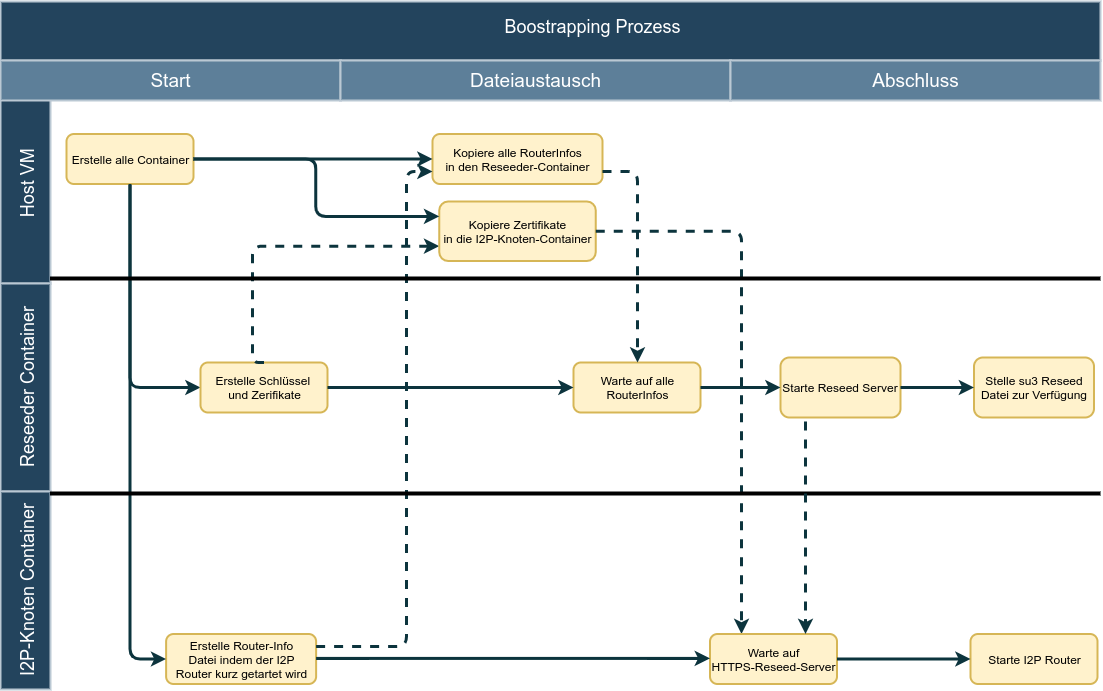
\includegraphics[height=0.85\textwidth]{bootstrap-diagram.png}
  \caption{Der Bootstrapping Prozess}\label{fig:bootstrap-diagram}
\end{figure*}
\end{landscape}% Landscape page


\subsection{Netzwerkisolation}

Während unserer Tests wollen wir nur Traffic unserer eigenen Knoten im Netzwerk und äussere Einflüsse vermeiden.
Dies um so gut wie mögliche und unbeeinflusste Messungen tätigen zu können.
Docker-compose respektive Docker bietet eine option ein internes Netzwerk zu erstellen,
welches einerseits vom Host nicht direkt erreichbar ist
und zudem die Container nicht auf das Host-Netzwerk zugreifen können.
Das folgende Quellcodelisting zeigt den Abschnitt für die Netzwerkkonfiguration wie deklariert in der \lstinline|docker-compose.yaml|.
Wichtig sind hier die Optionen \lstinline|driver: bridge| und \lstinline|internal: true|, die ein internes Docker-Netzwerk erstellen.
Die zusätzliche Option \lstinline|enable_icc| stellt sicher, das die Container jedoch untereinander kommunizieren können.
\begin{lstlisting}{language=yaml}
networks:
  i2ptestnet:
    name: $NETWORK_NAME
    driver: bridge
    internal: true
    driver_opts:
      com.docker.network.bridge.enable_icc: "true"
      com.docker.network.bridge.enable_ip_masquerade: "true"
    ipam:
      driver: default
      config:
        - subnet: 10.23.0.0/16
\end{lstlisting}

Zusätzliche Optionen zur Abgrenzung vom öffentlichen I2P-Netzwerk können in der \lstinline|i2pd.conf| spezifiziert werden.
Einerseits gibt es die Option \lstinline|netid|, diese ist Standardmässig auf die Nummer 2 gesetzt, da dies die Netzwerk-Id des öffentlichen I2P-Netzwerks ist.
Diese Option ist im Testnetzwerk jedoch zur Abgrenzung auf die Nummer 23 gesetzt. 
I2P-Router mit einer anderen Netzwerk-Id werden nie miteinander kommunizieren.
Diese Netzwerk-Id wird auch in den Router-Infos abgelegt werden auch nicht vom Reseeder 

Zudem gäbe es zum Testen im öffentlichen Netzwerk auch die 

Die Konfigurationsoption \lstinline|netid| erlaubt es die Netzwerknummer zu definieren.
Beim realen I2P-Netzwerk ist diese standardmässig auf \lstinline|2| gesetzt.

Für tests mit dem öffentlichen Netzwerk gäbe es zusätzlich noch die Option \lstinline|family|.

VM / Container, Konfigurationsoption \lstinline|nat|


\subsection{Adressbuch}

Standardmässig wird jeder Destination eine b32-Adresse gegeben.

Diese ist jedoch nicht einfach zu handhaben und anstatt es ist einfacher die Knoten direkt anhand ihrer Nummer zu adressieren.
Diese Adressen werden dann automatisch vom Socks5-Proxy der \lstinline|i2pd| mitliefert aufgelöst.
Damit kann das Messskript vereinfacht werden, da es dieses dann nicht die genauen Adressen zusammensuchen muss.

Auch wird die Auswertung damit vereinfacht weil, der TCP-Client den verwendeten Namen des TCP-Servers auch in die Nachricht hineinpackt und der TCP-Server diesen als Messausgabe abspeichert.
Es wird beim Startvorgang des Netzwerks für jede erstellte Destination für den TCP-Server ein Adressbucheintrag erstellt.
Dieses Adressbuch ist eine einfache CSV-Datei wird ebenfalls im Bootstrapvorgang an alle Knoten verteilt.
Im Falle von acht Knoten im Netzwerk sieht diese Datei beispielsweise so aus:

\begin{lstlisting}
tcpsrv-1.i2p,b2cdodoyqg5v6go56bkaevvw777e2wyiflqh6zyyyxugy4cqlzuq
tcpsrv-2.i2p,r6axddltht76mrtp5lrxtdxncilhgp7bcajkqtsj7l7fmoebgs3a
tcpsrv-3.i2p,ddhznqpxtgac7qa6yg6uzfpd55xoa2zfc4dwg4rh4qucx7veswlq
tcpsrv-4.i2p,3tyncnh7j4akqirrbdi4ek7nlysqmuvyav3ix326vwixvgoviz3q
tcpsrv-5.i2p,xj3qduyqur54v3mjgsxn6xa56q2ojyysf5n3bonpxyfxy5trnoja
tcpsrv-6.i2p,pt64eojrsvrp5w5izgwlide7j6vuw5td6g2pfrkurwsnmb4i7q2q
tcpsrv-7.i2p,aat6wqge3o7k2nabpwxrcu2vbbiydf3mj6n5k2zrrtozkrrpyfoa
tcpsrv-8.i2p,4wm4pqautqqb3a6yw3xif4zgwwu4v5tvpwv6onha27p5pkcqqepq
\end{lstlisting}

In der ersten Spalte ist der vereinfachte Name anzugeben und in der Zweiten Spalte die b32-Adresse, jedoch ohne die Endung \lstinline|.i2p|

\subsection{I2Pd-Container}

Hauptsächlich wird in diesem Container der \lstinline|i2pd|-Prozess ausgeführt.
Um andere Knoten zu kontaktieren zu können muss dieser zu Beginn den Reseed-Container anfragen nach einer Liste von RouterInfos.
Der TCP-Client und TCP-Server sind ebenfalls in diesem Container angesiedelt.
Dies verletzt zwar das Prinzip, dass man nur einen Prozess in einem Docker-Container ausführen sollte,
jedoch ist das Ziel hiermit Messungenauigkeiten aufgrund eines zusätzlichen Container zu vermeiden, sowie die Netzwerkkonfiguration zu vereinfachen.

\subsubsection{TCP Server Tunnel}

Diese Tunnel-Konfiguration führt dazu, dass I2P eine neue Destination mit einer .b32-Addresse erstellt.

Mit der folgenden Tunnel-Konfigurations-Datei wird der \lstinline|i2pd| konfiguriert, um einen TCP-Server-Tunnel zur Verfügung zu stellen:
\begin{lstlisting}
# serve some tcp service to others in the network
[tcp-in]
type = server
host = 127.0.0.1
port = 2323
keys = tcp-in.dat
gzip = false
enableuniquellocal = true
\end{lstlisting}

Hierbei gilt es zu beachten, dass die Schlüssel angegeben mit der \lstinline|keys|-Option, beim Aufstarten generiert werden.
Auch wurde mittels der Option \lstinline|gzip| die Komprimierung-Deaktiviert, damit auch wirklich die richtigen Nachrichten-Grössen übermittelt werden.

Die Option\lstinline|enableuniquellocal| wurde noch aktiviert, um die Auswertung zu vereinfachen. Denn diese führt dazu das der TCP-Server nicht immer dieselbe Ausgangsadresse \lstinline|127.0.0.1| bekommt, sondern je nach Sender der Nachricht eine andere \lstinline|127.0.0.0/8|-Adresse anhand der ersten Bytes des Public-Keys erhält. Jedoch wurde schlussendlich nicht auf diese Möglichkeit die Knoten zu identifizieren zurückgegriffen, da das Adressbuch 

%TODO: Reference config, especiallfor for enableuniquellocal.

\subsection{Nachrichten}

Die darüberliegende Blockchain-Schicht von diva.exchange versendet mittels eines Gossip-Protokolls die neuen Blocks der Blockchain an alle Knoten.
%TODO: add gossip protocol to glossary
Diese 64Kb grossen Blocks werden über eine Web-Socket-Verbindung an die Nachbarknoten übermittelt.
Die Nachbarknoten leiten diese dann wieder weiter an ihre jeweiligen Nachbarknoten.
Dieser Prozess wird solange wiederholt bis alle Knoten im Netzwerk den neuen Block erhalten haben.

Nach Absprache mit dem Auftraggeber wird dies im Testnetzwerk mittels versenden von TCP-Nachrichten nachgestellt.
Bei Web-Sockets handelt es sich vereinfacht ausgedrückt wiederum um eine TCP-ähnliche Verbindung über HTTP. HTTP selber TCP auch als Transportschicht.


\begin{itemize}
    \item Originator Node Id
    \item Destination Address
    \item Grösse der versendeten Nachricht in Bytes
    \item Zeitpunkt in nanosekunden seit 1.1.1970 
\end{itemize}


\subsubsection{Socks5-Proxy für den TCP-Client}

Dieser Socks5-Proxy ist der Gateway um innerhalb des I2P-Overlaynetzwerk zu kommunizieren.

Der folgende Ausschnitt aus der \lstinline|i2pd.conf| zeigt auf wie der Socks5-Proxy konfiguriert wurde:

\begin{lstlisting}
[socksproxy]
## Uncomment and set to 'false' to disable SOCKS Proxy
enabled = true
## Address and port service will listen on, like 127.0.0.1
address = 127.0.0.1
port = 4445
\end{lstlisting}

Zusätzlich wird in diesem Abschnitt auch die Länge der Tunnels bestimmt.

\subsection{TCP-Server}

Für Tests am Anfang wurde das Tool Netcat (kurz \lstinline|nc|) verwendet.
Dies hat gut funktioniert um die Konnektivität im Netzwerk zu testen. Hat aber zur effektiven messung einen Nachteil.

Um genauere Messresultate zu erhalten wurde eine e-poll basierte C-Implementation eines TCP-Servers erstellt, um die komplette Kontrolle über die Netzwerksocket zu bekommen.
Auch wurde C und nicht z.B. Python gewählt um den Arbeitsspeicher und CPU Gebrauch des Containers so tief wie möglich zu halten.
Dies erlaubt es die Latenz genauer zu messen und auch den TCP-Verbindungsaufbau nicht mitzumessen

Wie auch die Verbindung sofort nach Erhalt einer Nachricht wieder zu schliessen.

Auch erlaubt es nc nicht mehrere TCP-Verbindungen anzunehmen und die Verbindungen korrekt zu schliessen.

Der TCP-Server nimmt jeweils eine einzelne Verbindungen


\lstinline|docker/i2p/messenger/epoll-server.c|


\subsection{TCP-Client}

Damit der TCP-Client in das I2P-Overlaynetzwerk verbinden kann, muss dieser fähig sein mit einem Socks5-Proxy zu kommunizieren.
Zudem gilt es den Socks5-Proxy richtig zu konfigurieren.
Denn die Namensauflösung muss auch über I2P-Netzwerk abgehandelt werden.
Nur so können die \lstinline|.b32.i2p|-Adressen aufgelöst werden.
Ist diese im Addressbuch und hat diese eine zugehörige \lstinline|.b32.i2p|-Addresse.
Anhand einer \lstinline|.b32.i2p|-Adresse kann die netDb nach einem zugehörigen LeaseSet abgefragt werden, welches Zugriff auf die gewünschte Destination bietet.

Der TCP-Client ist ein kleines C-Programm welches in der 
i2p-testnet Repository in der Datei \lstinline|docker/i2p/messenger/client.c| zu finden ist.

Zusammengefasst macht es nichts anderes als
eine Verbindung mit einem Socks5-Proxy aufzubauen, und eine TCP-Nachricht der definierten grösse durch den Proxy versendet.

Es bietet folgende Kommandozeilenoptionen:

\subsection{Konfigurationsoptionen}

Diverse Konfigurationsopitionen wurden implementiert um verschiedene Tests durchführen zu können.
Jede der Optionen ist hier kurz beschrieben.

\begin{itemize}
    \item Anzahl Knoten im Testnetzwerk. Diese Option bestimmt wie viele I2Pd-Knoten ins Testnetzwerk eingebunden werden.
    \item Zu verwendendes I2Pd-Konfigurationsdatei.
    \item Reseeder Optionen:
        \begin{itemize}
        \item Anzahl RouterInfos pro Su3-Datei. welcher Knoten beim starten des Netzwerks kennt.
        \item Anzahl Verschiedene Su3-Dateien. Sets an RouterInfos. welcher Knoten beim starten des Netzwerks kennt.
        \end{itemize}
    \item Mess-Optionen:
        \begin{itemzie}
        \item Mess-Interval: 
        \item Anzahl Samples: 
        \item Nachrichtengrösse:
        \end{itemize}
\end{itemize}

Eine Beispiel \lstinline|config.json| könnte zum Beispiel so aussehen.

\begin{lstlisting}{language=json}
{
    "network": {
        "name":"network.i2pd.local",
        "private": true
    },
    "reseeder": {
        "router_infos_per_node": 48,
        "num_different_seed_files": 64
    },
    "nodes": {
        "amount": 64,
        "config_file": "conf/i2pd.org.conf",
        "bandwidth": [1000000]
    },
    "measurement": {
        "message_size_kb": 16,
        "num_messages": 1024,
        "sleep_interval": 6
    }
}
\end{lstlisting}

\subsection{Das Messskript}\label{sec:messskript}

Das Messskript ist dafür verantwortlich Nachrichten durch das Testnetzwerk zu senden, damit Messdaten erstellt werden.
Die Nachrichten werden von einem zufälligem Knoten zu einem anderen zufälligen Knoten verschickt.
Somit kann sichergestellt werden, dass die Latenzmessungen repräsentativ sind für das gesamte Netzwerk.
Um das Netzwerk nicht zu überlasten (siehe (TODO: ref)) werden die Nachrichten sequentiell versendet und es wird nur eine Nachricht auf einmal versendet.
Zudem wird nach jeder versendeter Nachricht wird 10 Sekunden gewartet.

Die Nachrichten werden versendet unter Verwendung von \lstinline|docker exec|.
Damit wird innerhalb des zufällig ausgewählten I2Pd-Containers ein TCP-Client-Prozess gestartet.
Dieser verbindet dann auf den Socks5-Proxy im gleichen Container.
Anschliessend schickt der TCP-Client die Nachricht der gewählten Grösse ins I2P Netzwerk.

Bevor das Messskript gestartet werden kann, müssen jedoch einige Bedingungen erfüllt werden.
Erstens muss mittels dem Recompose-Skript das Testnetzwerk in Betrieb genommen werden.
Zweitens muss gewartet werden, bis der Bootstrapping-Vorgang im Testnetzwerk abgeschlossen wurde.
Zu guter letzt muss noch einige Zeit gewartet werden und sichergestellt werden, dass das Netzwerk 
Dies ist um sicherzustellen, dass keine Messungenauigkeiten auftreten.
Einerseits gehen so keine Messpakete verloren. Andererseits könnten die Latenzmessungen verfälscht werden, wenn die Tunnels erst noch aufgebaut werden müssen.

Das Messskript ist in der i2p-testnet Repository in der Datei \lstinline|bin/measure-message-latency| zu finden.

\section{Testing}

CI? most don't allow this...

have a machine to deploy to

\subsection{BATS-Tests}

Diese Tests sind im Verzeichnis \lstinline|tests/| in der \lstinline|i2p-testnet|-Repository zu finden.

Um schnell zu prüfen, ob das Netzwerk korrekt konfiguriert wurde gibt es das Test-Modul \lstinline|tests/networking.bats|.
Dieses führt verschiedene Tests durch. Ob

\subsection{CI für den Bericht}

Dieser Bericht ist mit Hilfe von \LaTex umgesetzt.
Es handelt sich hier dementsprechend auch eine Art Programm darstellt mit einem Build-Vorgang.
Dieser Build-Vorgang wurde mit dem GitLab CI Service vom EnterpriseLab automatisiert.

\section{Benutzerhandbuch}

Dieser Abschnitt erklärt wie ein Tester selber neue Testnetzwerke erstellen, die Tests-Konfigurieren und selber Messungen tätigen kann.

\subsection{Deployment der Test-VM}

Wird NixOps verwendet 

\begin{lstlisting}{language=bash}
$ bin/recompose
\end{lstlisting}

Die verschiedenen


Alternativ kann auch jede andere Linux-Distribution mit oder ohne VM verwendet werden.
Wichtig zu beachten ist das folgende Software-Pakete installiert sind und mindestens die angegebenen Versionen (wo spezifiziert) verwendet werden:

\begin{itemize}
    \item docker-compose >= 1.28.2, verwendet für Container-Orchestration
    \item docker >= 20.10, verwendete Container-Technologie
    \item bash, benötigt da das \lstinline|recompose|-Skript und das Messskript in Bash geschrieben sind
    \item jq, Utility zum verarbeiten von JSON-Dateien
    \item moreutils, Weitere Shell-Utilities die vom \lstinline|recompose|-Skript verwendet werden (z.B. \lstinline|sponge|).
    \item bats, optional, wird benötigt um Selbsttests auszuführen
    \item sysstat, wird benötigt vom Messskript um die Ressourcenauslastung zu messen
\end{itemize}


\subsection{Konfiguration einer Messung}

Die Konfiguration der Messung kann in der \lstinline|config.json| angepasst werden.
Zusätzlich kann natürlich die Netzwerkkonfiguration der

\subsection{Erstellen des Testnetzwerkes}

Für alle folgenden Befehle wird davon ausgegangen, das ein Benutzer verwendet wird der Teil der \lstinline|docker| Gruppe ist und somit die Docker-Befehle ohne \lstinline|sudo| absetzen kann.

\begin{lstlisting}{language=bash}
$ bin/recompose
\end{lstlisting}


\subsection{Ausführen einer Messung}

Wird eine Messung mit 64 Knoten oder mehr durchgeführt muss die ARP-Neighbor-Tabelle des Hosts vergrössert werden, da der Standardwert  (siehe Schluss des Abschnitts~\fullref{sec:scaling}). Dies benötigt zwingend Root-Rechte da Kernel-Parameter verändert werden:

\begin{lstlisting}{language=bash}
# bin/networking-sysctls
\end{lstlisting}

Eine Messung kann wie folgt ausgeführt werden:

\begin{lstlisting}{language=bash}
$ bin/measure-message-latency
\end{lstlisting}
